% This is samplepaper.tex, a sample chapter demonstrating the
% LLNCS macro package for Springer Computer Science proceedings;
% Version 2.20 of 2018/03/10
%
\documentclass[runningheads]{llncs}

\usepackage[T1]{fontenc}
\def\doi#1{\href{https://doi.org/\detokenize{#1}}{\url{https://doi.org/\detokenize{#1}}}}
%
\usepackage{graphicx}

\graphicspath{ {figures/} }

\usepackage{amsmath,amssymb,amsfonts}
\usepackage{algorithm2e}
\usepackage{xcolor}
\usepackage{subcaption}


% Used for displaying a sample figure. If possible, figure files should
% be included in EPS format.
%
% If you use the hyperref package, please uncomment the following line
% to display URLs in blue roman font according to Springer's eBook style:
% \renewcommand\UrlFont{\color{blue}\rmfamily}
%
\usepackage{listings}
\lstset{language=Pascal}
% Please use the

\begin{document}
%
\title{Improving drift detection by monitoring Shapley Loss values}
%
%\titlerunning{Abbreviated paper title}
% If the paper title is too long for the running head, you can set
% an abbreviated paper title here
%
\author{Bastien Zimmermann\inst{1} \and
Matthieu Boussard\inst{1}\orcidID{0000-0001-5256-0462}}
%
\authorrunning{B. Zimmermann et al.}
% First names are abbreviated in the running head.
% If there are more than two authors, 'et al.' is used.
%
\institute{craft ai$^1$\\
\email{\{bastien.zimmermann  matthieu.boussard\}@craft.ai}}
%
\maketitle % typeset the header of the contribution
%
\begin{abstract}
%The abstract should briefly summarize the contents of the paper in
%150--250 words.
Along the deployment of Machine Learning models rises an inherent need for monitoring, where model performances should be tracked as well as potential drifts. In a live environment, with evolving data, the risk is for the model to become ill-adapted for the given situation.
The failure to detect drift while leading to a performance deterioration could also cause side effects due to model over-trust. Informing the user of any anomaly upon detection is the key to enabling any action.
We propose Shap-ADWIN, a novel approach improving the performance of state-of-the-art drift detectors such as ADWIN by leveraging the information brought by Shapley Loss Values.

While common practice is to monitor the evolution of the loss of models at most for every predicted instance, the proposed solution monitors each individual instance and features the Shapley Loss value. Whenever the loss is attributed more toward a given feature the information becomes more contrasted, which enables a better detection. Indeed the signal-to-noise ratio is higher on that feature and allows the detector to leverage that information. The opposite case being equal Shapley values that are just the Loss under-scaled for every feature. Moreover, noise over the output would be equally distributed along with each Shapley Loss value of every feature providing lower information to noise ratio and allows a more reliable detection. We provide: a restricted proof, experiments and source code. Results were obtained using synthetically generated data presenting diverse types of drift, showing the performance of Shap-ADWIN over ADWIN.

\keywords{Shapley values  \and Drift-detection \and ADWIN}
\end{abstract}
%
%
%
\section{Introduction}
With the general development of Artificial Intelligence (AI) and Machine Learning (ML) algorithms, the risk for AI applications to encounter edge cases in which the systems perform or react in an unplanned or unexpected way rises. Consequently, it becomes essential to monitor the deployed models, that is to say, control the performances and impacts of the system in its environment.
One major problem is unstable data dependencies, \cite{hiddenTechnicalDebtsinMLSsculley} as some inputs signals are unstable as they qualitatively and/or quantitatively change behavior over time.
%When it comes to the learning target if the statistical properties of that label change over time it is called concept drift.

All these evolutions can induce a performance degradation, the model being ill-suited to new environments or events. ML solutions facing drifts have to change, re-adapt themselves as the solution they offer is no longer relevant.
Drift monitoring presents three main challenges: identifying important changes over the data distribution, identifying the inadequacy of the ML model with respect to its context, and identifying key points to leverage in order to get the model back on track. Our study is focused on the first challenge: Determining when the underlying data distribution suddenly changes into a different one and hinders the model's behavior. While any unforeseen or unexpected change in the data is relevant in most cases, the point of interest is the model behavior. Although common approaches monitor the input data and the model loss separately, \cite{lundberg2020local2global} presents the decomposition of the loss among the model's input features in order to improve problems identification and debugging.

In this article, we introduce Shap-ADWIN (Section \ref{Detect Shap Vals}), a novel algorithm to better detect this phenomenon. It combines interventional Shapley values and the Adaptive Windowing drift detector \cite{bifet_learning_2007} in order to produce a more reliable and efficient detection. After computing the Shapley values, a detector is fed each feature Shap-Loss values. There is one Drift detector per feature, each dealing with the loss attribution for every value taken by this feature.
Experimental results point that the newly introduced algorithm detects the drift more often and earlier compared to the alternative without Shapley values. 
%TODO: Check if tronconne CAN BE TR
Drifts can have many different characteristics, they may occur in the feature distributions, in the label distribution or it can even be the underlying concept learned that is changing. Furthermore, each one of these drifts may occur differently, with diverse patterns. A drift might be very sudden, abrupt or it may appear gradually. Accordingly to this diversity, our experimental setting is based around the generation of synthetic datasets presenting various drifts cases. Across the majority of the studied scenarios, Shap-ADWIN is shown to perform better compared to ADWIN w.r.t the metrics exposed. The code used for the experiments is available in a Github repository and can be found as supplementary material.   \textcolor{blue}{\underline{\url{https://github.com/craft-ai/shap-adwin}}}

After first exploring related work on Drift Detection and Shapley values, we introduce our novel drift detector Shap-ADWIN. Along with the intuition behind the functioning of our approach a restricted mathematical proof is provided. Further on, experimental results are presented demonstrating the improvement brought by Shap-ADWIN over ADWIN and the impact on the detection of: the Shapley values background set, noise on the target label, and the variation of the detector hyper-parameter.

\section{Related Work}

    \subsection{Drift Detection}
    %A data stream is a sequence of data points continuously observed over time. The specificity of this format is the ability of the signal to change over time. 

    Calling \emph{concept} the learned target, a \emph{concept drift} is any change of the underlying data distribution. 
    %ML models which are learning from data streams observe their performance declining over time as the assumption of the training data being representative of the live environment is not satisfied anymore. 
    %Concept drift comes in different types and characteristics. 
    Drift velocity, severity, and patterns vary, designated as abrupt when the distribution transition is sudden or gradual when it changes progressively, it is incremental when the probability that observed instances belong to the new concept increases over time while the probability of the ones belonging to the previous concept decreases. 
    %ML models which are learning observe their performance declining over time as the assumption of the training data being representative of the live environment is not satisfied anymore. 
    %However, a detector should be stable; blips (abrupt drift with very short concept duration) or outliers detection is left to the user to decide as they might not be detection-worthy. %While adjusting a system to blips is debatable, outliers should not be of any influence.
    %Although well-designed and properly tuned ML models should overcome noise, they are not intended to overcome drifts. Indeed, the assumption of the training data being representative of the live environment is not satisfied anymore. A Drift detector is thus needed.
        
        
    Over the different characteristics, drifts can be grouped into different types. \cite{souza_challenges_2020} identifies the three types of drifts:
    \begin{itemize}
    \item A \emph{Covariate Drift}: The input distribution changes over time. 
    \item A \emph{Prior probability shift}: The output distribution changes over time
    \item A \emph{Concept shift} The relation between input and output changes over time.
    \end{itemize}

    
    
    In order to determine when those drifts occur, and doing so the fastest way possible, different drift detection methods exist. 
    Obtaining this information is the keystone to any adaptation mechanism.
    %WITH citations
    %Four types of drift detection methodologies exist \cite{gama_survey_2014}.
    %These methods are based on either: Sequential analysis \cite{pagehinkley}, Control Charts \cite{EDDM}, Monitoring of two distribution \cite{bifet_learning_2007} or Contextual.
    %Without
    Four types of drift detection methodologies exist \cite{gama_survey_2014}.
    These methods are based on either: Sequential analysis, Control Charts, Monitoring of two distribution or Contextual.
    
    The evaluation of drift detectors can be made through many domain-dependant points of view. Not all drift detectors respond to the same requirements, thus evaluation metrics may differ.
    When dealing with well-identified drift, for instance when using synthetic datasets, the detector's performance can be measured through earliest detection, detection frequency, and mean duration until detection. These metrics allow clear and comparable results.
    
    
    A classical robust detector is the ADaptive WINdowing drift (ADWIN) detector \cite{bifet_learning_2007}. Through the monitoring of differences between distributions and the sliding window, it aims to the optimal window to handle best the concept drift. While old samples should be discarded as they aren't representative anymore, they might still be representative of an important learning aspect. Adjusting the window is one example of handling the stability-plasticity dilemma.
    The algorithm automatically adjusts the size of the window to keep a sufficient enough number of samples to detect a significant enough change in means. 
    
    ADWIN has a unique parameter \cite{gomes_adaptive_2017}: the confidence level $\delta$ making it robust as there is no possibility of ill-tweaking other parameters. This real value between 0 and 1 impacts directly the cut threshold $\epsilon_{cut}$ this is the detection threshold. Moreover, as exposed by \cite{souza_challenges_2020} ADWIN reaches some of the best results on benchmark data representative of many different drifts.

\subsection{Shapley Values}
    In 1951 Lloyd Shapley introduced the Shapley Value as a solution to distribute the total value of a coalition to each player's contributions. It is a \emph{"fair"} manner of sharing the payout of a game. 
    The Shapley values $\phi_i(v)$ for a game $v$ are the unique allocations that satisfy the following properties: With $N$ the set of all players, $S$ a given coalition of players, $v$ the game-defining value function, $\phi_i$ Shapley value for player $i$.
    
    \begin{enumerate}
        \item \textbf{Efficiency:} The allocations add up to the difference in value between the grand coalition and the empty coalition.
        \begin{equation}%TODO: Check whether we can reduce the equation size
            \label{eq: Efficiency}
                \sum_{i \in N}{\phi_i(v) = v(N) - v(\{\varnothing\})}
        \end{equation}
        
        \item \textbf{Monotonicity:} If a player $i$ increases a game $v$ value more than they would for game $v'$ for all possible remaining sets of players, then $i$'s attribution for $v$ should be greater than or equal to his attribution in $v'$. 
        
        %\begin{equation*}
        %\label{eq: Monotonicity}
        %\begin{aligned}[l]
        %    v(S \cup  \{i\}) - v(S) \geq v'(S \cup i) - v'(S) \; \forall S \subseteq N \setminus i \\
        %    \implies \phi_i(v) \geq \phi_i(v')
        %\end{aligned}
        %\end{equation*}
        
        \item \textbf{Symmetry:} Two players $i,j$ that make equal marginal contribution to all coalitions receive the same allocation.
        %\begin{equation*}
        %    v(S \cup  \{i\}) = v(S \cup  \{j\}) \; \forall S \subseteq N \setminus i,j \Rightarrow \phi_i(v) = \phi_j(v)
        %\end{equation*}
        
        \item \textbf{Dummy:} A player $i$ making 0 marginal contribution receives 0 allocation.
        %\begin{equation*}
        %\label{eq: Symmetry}
        %    v(S \cup  \{i\}) = v(S) \; \forall S \subseteq N \setminus i  \; \phi_i(v) = 0
        %\end{equation*}
        
        \item \textbf{Linearity:} For two games v and v' and their respective allocations $\phi_i(v)$ and $\phi_i(v')$, then the cooperative game defined as their sum $v = v'$ has allocations defined as the sum of each game's allocations.
        \begin{equation}
        \label{eq: Linearity}
            \phi_i(v + v') = \phi_i(v) + \phi_i(v')
            \; ; \; \phi_i(av) = a \phi_i(v)
        \end{equation}
    \end{enumerate}
    
    Thanks to those desirable properties, the Shapley values have been widely used in different contexts, notably in Artificial Intelligence. They can provide an estimation of the contribution of an algorithm to a portfolio, data valuation for a machine learning model, model agnostic approach to explain the output of machine learning models, \cite{NIPS2017_7062},
    global feature contribution with additive importance measures \cite{SAGE_covert}, feature selection or even explaining non-linear model output transformations (such as the model’s loss) \cite{lundberg2020local2global}.
    
    This unique allocation, the Shapley value for the feature $i$ of the game $v$ takes the following form:
    

    \begin{equation}
        \phi_i(v) = \sum_{S \in N \setminus \{i\}}\frac{|S|! (|N|-|S|-1)!}{|N!|} {(v(S \cup i) - v(S))}.
    \end{equation}
    It is the average marginal contribution of that player for all possible permutations of remaining players:
    
    \subsection{Shapley values for machine learning}
    
    Oppositely to the game-theory case it is not possible to assign credit for a ML model through Shapley values directly as most models require inputs with values for every feature, rather than a subset of features. %\cite{Chen et al 2021 Explaining a series of models by propagatin Local ....}
    To obtain local feature attribution it is required to define a set function $v(S)$ that is a \emph{lift} of the original model $f(x):\mathbb{R}^m\rightarrow\mathbb{R}^1, m\in \mathbb{N}$ \cite{Merrill2019GeneralizedIG,Chen_attributions}.
    In this context we assume the model to be a game where each feature is a player, the value of the game is the model output and the rules are defined by the representation learned by the model. 

    \noindent While the choice of the lift is influential, the Shapley values computed throughout this study will use the 
    \emph{interventional conditional expectation}:
    \begin{equation}
        v(S) = \mathbb{E}_D[f(x)|do(X_S)].
    \end{equation}

    
    \noindent J. Pearl $do$ operator for causal inference breaks the dependence between features \cite{Janzing2020FeatureRQ}. It requires a background Distribution $D$ (cf sec. \ref{section:background}) that the foreground, sample to explain $x^f$ will be compared to. For a single background instance $x^b$:
    
    \begin{equation}
    \mathbb{E}_D[f(x^f)|do(x_S)] = f(h^S),       
    h^S_i =\begin{cases}
    x_i^f &\text{if $i \in S$}\\
    x_i^b &\text{otherwise}
    \end{cases}
    \end{equation}
    
    
    \begin{equation}
        \phi_i(f,x^e,D) =  \frac{1}{|D|}\sum_{x^b \in D}\phi_i(f,x^e,x^b).
    \end{equation}

    This interventional approach is described to better reflect the model behavior \cite{chen_true_2020}, yet it can lead to computing Shapley values on points that are away from the true data manifold \cite{frye2020asymmetric}. TreeSHAP detailed in \cite{lundberg2020local2global} allows to compute quickly and exactly the interventional Shapley values for tree based algorithms. 
    
    
\subsection{Shapley Loss Values}
    Loss attribution through Shapley values provides different insights in comparison to the model output alternative. The interventional approach using a background distribution allows us to explain non linear transformations of the model output such as the loss.
    These local feature attributions that explain the per-sample loss
    can be used to identify the impact of a covariate shift with feature attributions \cite{Chen_attributions} or signal problems that would have been hidden \cite{lundberg2020local2global}.
    
    It defines as important the features whose absence degrades the model performances through this notion of predictive power of feature subsets (difference between the mean prediction and the one over features in our subset).

    Given a loss function $l$, an instance $x$ and its label $y$ the reduction in risk over the mean prediction is defined as follow \cite{SAGE_covert}:

\begin{equation}
    v_{f,x,y}(S) = l(f_{\text{\o}}(x_{\text{\o}}),y) - l(f_{S}(x_{S}),y).
\end{equation}


\section{Shap-ADWIN: Drift detection on Shapley values}\label{Detect Shap Vals}

In order to improve the performance of a drift detector, we leverage the Shapley values loss attributions. 
By assigning a single detector to every single feature it monitors the feature Shapley loss values for each instance.

%WHY CHOOSING ADWIN ->
In this context, the signals seen by the detectors are continuous, even for classification problems the observation is focused on the log-loss resulting from the model output likelihood.
Aside from the continuous constraint our method is detector agnostic. While we don't rely on any specific aspect, ADWIN is convenient as it simplifies the parameter-tuning task by relying on a single hyper-parameter ($\mathbf{\delta}$) and performs well in many scenario. The ADWIN detector algorithm can be found in the appendix or in \cite{bifet_learning_2007}. %TODO: add ADWIN to the apendix 

In the following algorithm $Ad_i$ indicates the ADWIN detector receiving the Shapley values of the feature $i$, '\textit{raises a Detection}' is used to indicate the detector returning a positive output signaling a Drift. 
$\phi_i(x)$ designates the Shapley Loss value of Feature $i$ of the instance $X$. The computation of those values can be obtained with the TreeShap algorithm for a LGBM model using the logloss.

\begin{algorithm}[htbp]
        \DontPrintSemicolon
        \KwResult{Shap-ADWIN}
        \For{each feature $i$}{
            Initialize $Ad_i$ an ADWIN detector on feature $i$ 
        }
        \For{each instance $x$} {
            compute $\phi(x)$ Shapley Loss Values of instance $x$
            \For{each feature $i$} {
                Update $Ad_i$ ADWIN detector with $\phi_i(x)$ 
                
                \If{ $Ad_i$ raises a Detection} {
                    output Detection}
            }
        }
        \caption{The Shap-ADWIN algorithm}
        \label{alg:shap-ADWIN}
    \end{algorithm}
    
The complexity at each instance is
\begin{equation}
     \mathcal{O}(\,
    \underbrace{(|D|\times(\#Nodes)\times(\# trees))}_\text{TreeShap, D: Background set } + 
    \underbrace{log(W)}_{\text{ADWIN}}
    \times(\#feat)).
\end{equation}

    

\subsection{Intuition}%Theoretical hindsight

    Due to the nature of Shapley loss values and the Symmetry axiom (cf $2.2$), one could argue that the impact of noise on the loss should be the same across all features. 
    As the detector leverages the information and ignores the noise, the bigger the ratio of information to noise the better the detector performs. The noisier the signal the more difficult it gets for scale-independent detectors to identify the occurrence of potential drifts.
    %The more noise there is the higher the loss. 

    Suppose now that the noise impact is uniform across all features, i.e. the loss increases uniformly with noise regardless of which feature it is from. Any discrepancy in information on a feature would be differently dispatched through Shapley values, whereas, the noise effect would be equally shared across every feature.
    The worst case being when the feature having equal contributions then the attributions would be a de-scaled version of the overall loss, any scale independent detector would then perform equally well.

\subsection{Mathematical foundations}
Let's suppose that our model cannot learn from the noise $\epsilon$ and that our loss function $f$ takes the following form: With $F$ the set of features

\begin{center}
    $f(x+\epsilon) = g(x)+h(\epsilon) \text{ , Where: } h(\epsilon) = \sum_{i\in F}{\epsilon_i}$
\end{center}

Thanks to the Linearity property of Shapley values (Eq.\ref{eq: Linearity}), the Shapley value for the loss on feature $i$ is:
$$\phi_{i,f}(x+\epsilon)= \phi_{i,g}(x) + \phi_{i,h}(\epsilon) = \phi_{i,g}(x) + \epsilon_i$$

We then define the following information to noise ratios for respectively Shapley values $\phi$ and the loss $f$:
$$R_{\phi_i} = \frac{\phi_{i,g}}{\epsilon_i} ; 
R_{f} = \frac{g(x)}{\epsilon} \text{ , Where: } \epsilon = \sum_{i \in F}{\epsilon_i}; \epsilon_i, \epsilon \in \mathbb{R}^*
$$
%\begin{theorem} Let
%\[\forall i \in F,\; \epsilon_i = \frac{\epsilon}{n} \quad with \quad \epsilon \in \mathbb{R}^*  \; and \; n = |F|, \]There is at least one feature k for which:
%\[
%R_{\phi_k} \geq R_f
%\]
%\end{theorem}
\begin{theorem} Let $i \in F,\; \epsilon_i = \frac{\epsilon}{n}$ with $ \epsilon \in \mathbb{R}^* $ and $n = |F|$
$$
\exists k \textrm{ such as } R_{\phi_k} \geq R_f
$$
\end{theorem}
\begin{proof}
Thanks to the efficiency property (Eq.\ref{eq: Efficiency}) we can write:
\[\frac{g(x)}{\epsilon}=\frac{\sum{\phi_{i,g}}}{\epsilon}\]
\[\exists k, R_{\phi_k} \geq R_f \iff \exists k, \frac{\phi_{k,g}}{\epsilon_k} \geq \frac{\sum_{i \in F}{\phi_{i,g}}}{\epsilon}\]
Depending on the sign of $\epsilon$  we can chose either $max(\phi)$ or $min(\phi)$ as index k.
\end{proof}

Whenever this inequality is verified, a drift detector will perform better on a feature Shapley-Loss attributions. (Cf $3.1$)% as the information is less blurred compared to the overall loss.

With a more general definition of the noise (removing the $\forall i \in F,\; \epsilon_i = \frac{\epsilon}{n}$ constraint), it is possible to show that:
the ratio between the discrepancies among Shapley values and the discrepancies among noise values being bigger than the ratio of a given feature $k$ Shapley value and its noise is sufficient to have: $
R_{\phi_k} \geq R_f$.
Having bigger discrepancies among Shapley values than discrepancies among noise values is sufficient to ensure a better ratio on one feature Shapley value.




\section{Experimental Results}

Most experiments are based on a synthetically generated circle dataset. This dataset is defined using a fixed number of features where for each point each feature value is randomly sampled. The labels are generated by a hyper-sphere, if the point is inside the label is True otherwise False, this is our circle concept. Note that this simple concept is convenient as it cannot be perfectly learned by tree based models due to its curved nature.


The data is generated in two steps. First is the feature generation; with a default number of three, for each feature, the values are sampled from a uniform distribution over $[0, 1)$. The second is setting the decision boundary; each instance is checked to be inside or outside of the decision boundary (hyper-sphere) and the label is respectively set to "True" and "False". 

That generative process is then modified to incorporate a drift pattern in it. 
\begin{enumerate}
    \item \textbf{Abrupt Concept Drift:} At index $i$ change the hyper-sphere decision boundary to other parameters (center coordinates and radius). 
    \item \textbf{Gradual Concept Drift:} From index $i$ to index $i+Width$ move the hyper-sphere decision boundary center by $\delta_t= \frac{center_B - center_A}{Width}$ at each step.
    \item \textbf{Covariate Drift:} For a given feature and a given zone (range of indexes) limit the feature values to be sampled from a uniform distribution over [a,b), where $a>=0$ and $b<=1$
\end{enumerate}

By default, any part of the generated data that is not modified by any drift pattern is assigned a hyper-sphere of $center=(0.4, 0.4, 0.4), radius = 0.25$ in 3 dimensions as a default decision boundary. For each Drift case the change can be applied along a single axis or using all available dimensions.

%%TODO: CHECK IF TRONçonnable
The other datasets used are classical methods taken from the drift literature:
\begin{enumerate}
    \item \textbf{Sine1} (Abrupt concept drift): Two attributes $x$ and $y$ uniformly distributed in $[0, 1]$. The class is define according to $y = sin(x)$ positive if under the curve; negative otherwise. At a drift point, the class labels are reversed.
    \item \textbf{Sine2}: Identical to Sine1 with $y = 0.5 + 0.3 * sin(3 \pi x)$.
    \item \textbf{Stagger} (with abrupt concept drift): This dataset contains three nominal attributes, namely \emph{size}, \emph{color}, and \emph{shape}. The positive decision shifts from [\emph{color = red} and \emph{size = small}] to [\emph{color = green} or \emph{shape = circular}].
\end{enumerate}
 
Without loss of generality, the model used is LGBMClassifier \cite{lgbm} with default parameters to use Tree-SHAP and minimize computational costs by having efficient computation of exact Shapley values. 


Each detector performance is evaluated using: False and True positive rates (FP, TP) of detection, Min, Mean, Median, Max, and standard deviation (STD). The aforementioned metrics are the respective statistical function computed on several drift detection simulation e.g. the mean detection over 50 iteration of ADWIN on the Sine1 dataset. The unit is the number of instances and the origin is the drift starting point. 


\begin{figure*}[htbp]
\begin{center}
    \begin{tabular}{|l|r|r|r|r|r|r|r|r|}
    \hline
   \textbf{Drift} & \textbf{Method} &  \textbf{FP} & \textbf{TP} & \textbf{Min} & \textbf{Mean} & \textbf{STD} & \textbf{Max} & \textbf{Median} \\
    \hline
    
    
\textit{Gradual Concept - A} & \textbf{SHAP} &                     0.01 &                    1.0 &                    459 &                  1686 &                      236 &                   2187 &                  1675 \\ \cline{2-9} {} & ADWIN &  \textcolor{green}{-0.01} &  \textcolor{red}{-0.24} &  \textcolor{green}{-64} &  \textcolor{red}{+976} &  \textcolor{red}{+300} &  \textcolor{red}{+2208} &  \textcolor{red}{+992} \\ \hline
 \textit{Gradual Concept - B} & \textbf{SHAP} &  0.0 &  1.0 &                   779 &                  1501 &                     201 &                  1931 &                  1451 \\ \cline{2-9} {} & ADWIN & =\; & =\; &  \textcolor{red}{+576} &  \textcolor{red}{+326} &  \textcolor{red}{+58} &  \textcolor{red}{+608} &  \textcolor{red}{+368} \\ \hline\hline
 
 \textit{Abrupt Concept - A} & \textbf{SHAP} &                    0.0 &                    1.0 &                    75 &                    307 &                       77 &                    459 &                    331 \\ \cline{2-9} {} & ADWIN &  \textcolor{red}{+0.01} &  \textcolor{red}{-0.06} &  \textcolor{red}{+192} &  \textcolor{red}{+1312} &  \textcolor{red}{+821} &  \textcolor{red}{+2752} &  \textcolor{red}{+1120} \\ \hline
 \textit{Abrupt Concept - B} & \textbf{SHAP} &  0.0 &  1.0 &                    107 &                   323 &                       76 &                    523 &                  331 \\ \cline{2-9} {} & ADWIN & =\; & =\; &  \textcolor{green}{-32} &  \textcolor{red}{+152} &  \textcolor{red}{+193} &  \textcolor{red}{+1728} &  \textcolor{red}{+64} \\ \hline\hline
 
 \textit{Abrupt Covariate - A} & \textbf{SHAP} &  0.0 &                    1.0 &  119 &                   289 &                      147 &                   1399 &                  279 \\ \cline{2-9} {} & ADWIN & =\; &  \textcolor{red}{-0.01} & =\; &  \textcolor{red}{+131} &  \textcolor{red}{+178.00} &  \textcolor{red}{+1248} &  \textcolor{red}{+96} \\ \hline
 \textit{Abrupt Covariate - B} & SHAP &  0.0 &  1.0 &   23 &                    73 &                        28 &                    183 &     55 \\ \cline{2-9} {} & \textbf{ADWIN} & =\; & =\; & =\; &  \textcolor{green}{-8} &  \textcolor{green}{-11.00} &  \textcolor{green}{-96} &   =\; \\ \hline\hline
 
 \textit{Stagger - single Drift} & \textbf{SHAP} &  0.0 &  1.0 &                  103 &                 159 &                        16 &  167 &    167 \\ \cline{2-9} {} & ADWIN & =\; & =\; &  \textcolor{red}{+64} &  \textcolor{red}{+8} &  \textcolor{green}{-16.00} & =\; &   =\; \\ \hline
 \textit{Sine 1 - single Drift} & \textbf{SHAP} &  0.0 &  1.0 &                   71 &                   71 &    0 &                   71 &                   71 \\ \cline{2-9} {} & ADWIN & =\; & =\; &  \textcolor{red}{+32} &  \textcolor{red}{+32} & =\; &  \textcolor{red}{+32} &  \textcolor{red}{+32} \\ \hline
 \textit{Sine 2 - single Drift} & \textbf{SHAP} &  0.0 &  1.0 &                   39 &                   47 &                        21 &                    103 &                   39 \\ \cline{2-9} {} & ADWIN & =\; & =\; &  \textcolor{red}{+32} &  \textcolor{red}{+24} &  \textcolor{green}{-21.00} &  \textcolor{green}{-32} &  \textcolor{red}{+32} \\ \hline


    \end{tabular}
 \caption{\label{tab:Table 1}Shap-ADWIN and ADWIN drift detector relative performances facing Drift.
 (A: single feature drift, B: all features drift)}
\end{center}
\end{figure*}

%Maybe PARTLY redundant with metrics Section
\vspace{10pt}

Overall results are presented in Fig.\ref{tab:Table 1}.
The methods are ranked based on TP then Median, Mean, and STD. For each row-pair the best performing method is in bold. $+, -, =$ indicate the relative performance with respect to the other method, the colors green and red indicate respectively a better and a worse relative performance. The unit is in number of instances. 

The Shap-ADWIN drift detector outperforms ADWIN in all but one Drift scenario (cf. Fig.\ref{tab:Table 1}). 
Drifts impacting a single feature increase the performance discrepancies between Shap-ADWIN and ADWIN compared to drift on all features. When the drift is localized on a single variable all indicators present bigger discrepancies, except minimum detection in the gradual concept drift case.
The worst-case makes Shap-ADWIN slightly less stable with a higher standard deviation and higher mean detection, however, the median detection is equal i.e. in half of the cases both approaches detect the problem before the same median point (Fig.\ref{fig:Worst case}). This occurs for an Abrupt Covariate Drift on all features, all other scenarios present Shap-ADWIN as the better alternative.

%THIS does not comment the table
%On each figure, violins present the probability density at different values smoothed by a kernel density estimator. The three black vertical markers attached to the violin correspond to the minimum, median and maximum values. 

\begin{figure}[htbp]
     %\begin{subfigure}[b]{0.98\textwidth}
        \centering
        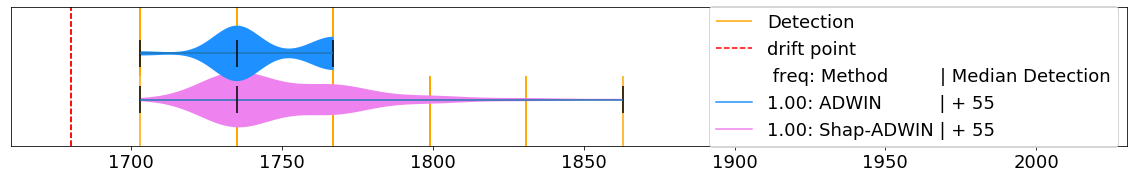
\includegraphics[width=0.9\linewidth]{worse_violin.png}
        % \caption{}
     %\end{subfigure}
    %\begin{subfigure}[b]{0.98\textwidth}
    %     \centering
    %    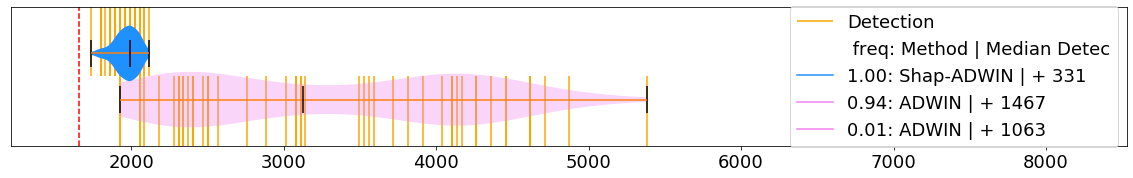
\includegraphics[width=\linewidth]{best_violin.png}
    %%     \caption{Abrupt Concept Drift on a single feature (Best case for Shap-ADWIN)}%TODO: FIX CAPTION
     %    \label{fig:Best case}
     %\end{subfigure}
        \caption{Detection Distribution per detector over 50 iterations\\
        Covariate Abrupt Drift on all features (Most competitive case)
        \\ (violins present the probability density smoothed by a kernel density estimator)%(1 bar is 1 detection for 1 iteration, the violin is the overall distribution)
        }
        \label{fig:Worst case}
\end{figure}
\subsection{Background dataset}
\label{section:background}
Interventional Shapley Values require a background dataset for their computation. This set of points is estimated to represent the prior over our data. Common practice is to sample at random a sufficient amount of points and it provides sound results. To investigate the impact of different background sets on Drift detection, 4 heuristics were developed where each background is filled picking from a pool of consecutive instances in the training set: \textbf{Small background:} 2 points at random, \textbf{Best background:} 10\% lowest loss points, \textbf{Worse background:} 10\% highest loss points, \textbf{Random background:} 10\% points at random.

\begin{figure}[htbp]
    \begin{center}
    \begin{subfigure}[b]{0.98\textwidth}
        \centering
        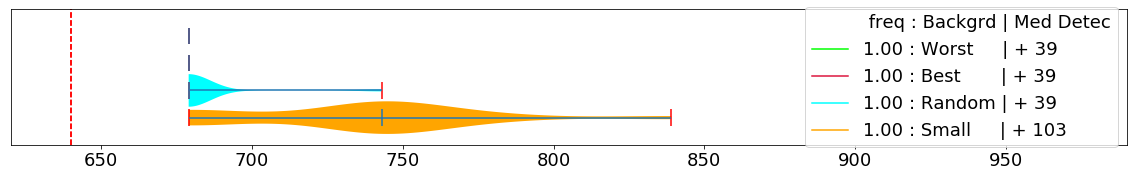
\includegraphics[width=0.9\linewidth]{bgrd_violin.png}
        \caption{Background impact on detection distribution - Sine2 dataset - ShapAdwin}
        \label{fig: Detection Background}
    \end{subfigure}
    \begin{subfigure}[b]{0.98\textwidth}
        \centering 
        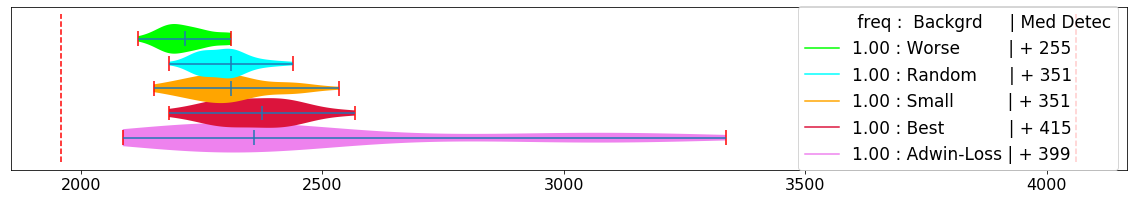
\includegraphics[width=0.9\linewidth]{bgrd_worse_best.png}
        \caption{Background impact on detection distribution - Circle abrupt concept Drift}
        \label{fig: Bgrd WorseBest}
    \end{subfigure}
    \caption{Background Heuristics Impact on detection}
    \end{center}
\end{figure}

Results Fig.\ref{fig: Detection Background} was generated using a Sine2 dataset comporting a single abrupt concept drift. The background choice is the only varying factor, in this case it has a very small impact. Picking values under-representative of our data such as outliers can lead to worse performances the small backgrounds do not contain sufficient information and the resulting average detection takes longer.

%%BEST VS WORSE.

Best and Worse background filling methods results are sensibly different compared to the random alternative. Changing the information in the background dataset that represents our prior does have an impact on the distribution of the resulting Shapley values. Coincidentally, the Best background performs relatively better than its alternatives Fig.\ref{fig: Bgrd WorseBest}. 

%Can be tronconned as scatter figure was removed
%As it is confirmed by Fig.\ref{fig: pre-post bgrd} the lowest Shapley values vastly disappear in the \emph{Best} case making the pre and post-drift distribution more contrasted than its \emph{Worst} alternative. The lower the Shapley value, the better the attribution is.
Finding efficient methods to fill the background could save many resources as TreeSHAP complexity is linear in terms of background samples and it is used at every sample. For a stable stream that drifts rarely a small efficient background would be highly beneficial. 







\subsection{Influence of noise on Drift Detection}
To investigate the impact of noise, we flipped at random $5\%$ of labels in the dataset. Fig.\ref{fig: noise_violin} Compare the performances on the same dataset with and without noise for both detectors. For Shap-ADWIN the noise has no impact on the detection rate and a small increase in detection latency is seen. ADWIN fails to detect reliably in a noisy context and the detection latency increases significantly. Our method is particularly fitted to overcome this kind of noise.

\begin{figure}[htbp]
    \begin{center}
        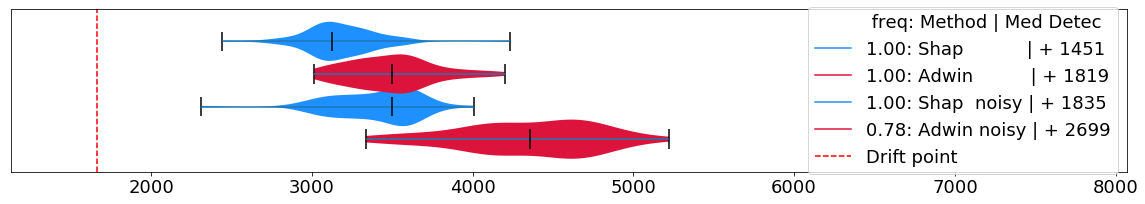
\includegraphics[width=0.9\linewidth]{noise_violin.png}
        \caption{Noise impact on detec distrib;Gradual concept drift on all feat.\centering($\delta = 0.01$)}
        \label{fig: noise_violin}
    \end{center}
\end{figure}

%------------------------------------------------------------------------------
\subsection{Influence of sensitivity of the detector}
We investigate the influence of the $\delta$ hyper-parameter for the drift detector ADWIN. The confidence level indicates the sensitivity selected for the detector, the higher the more confident the detector is.

\begin{figure}[htbb]
    \begin{center}
        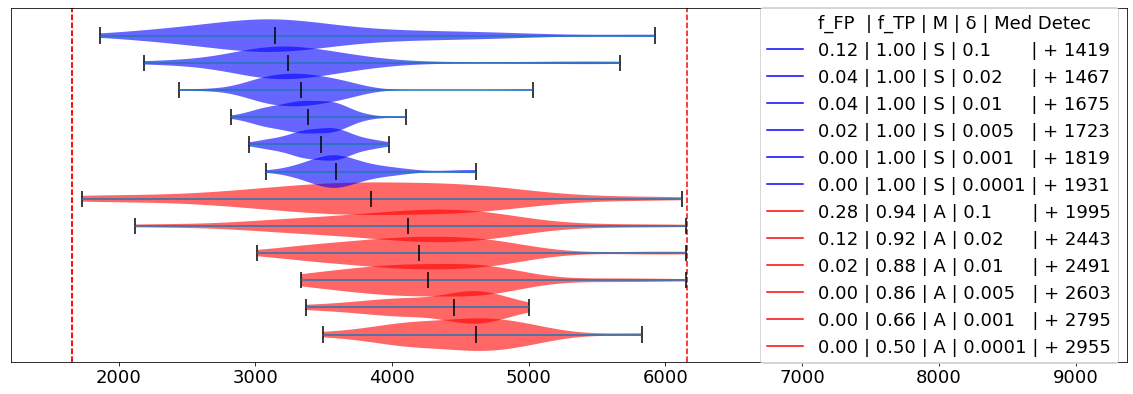
\includegraphics[width=0.9\linewidth]{beta_violin.png}
        \caption{Impact of ADWIN $\delta$ on Detection Distribution (\textbf{S}: Shap-ADWIN,\\ \textbf{A}: ADWIN, \textbf{f\_FP}: freq False Positive, \textbf{f\_TP}: freq True Positive)}
        \label{fig: beta violin}
    \end{center}
\end{figure}

Fig. \ref{fig: beta violin} is generated comparing ADWIN and Shap-ADWIN detection policies for several values of $\delta$, re-generating the dataset (gradual concept drift - CIRCLE on all 3 features and a transition period of 2000 instances) several times.
%Each Violin corresponds to the detection distribution for one method and one $\delta$ value. 
The top section presents the false detection i.e. occurring before the drift appearance. The bottom one contains true detection.

Within the range of $\delta$ tested, Shap-ADWIN is better than any ADWIN as it has and earlier, more reliable and more consistent detection. 
High $\delta$ values cause some false detection, however, there is no clear difference between Shap-ADWIN and ADWIN here, the choice of $\delta$ has more impact than the method chosen.
Here, Shap-ADWIN is better than ADWIN regardless of any $\delta$ choice.

\section{Conclusion} 
Combining the strength of drift detectors with Shapley values provides a more reliable and more stable drift detection. The new approach proposed monitors the loss on each feature for a ML model with an ADWIN drift detector fed with Shapley Loss values. We showed that this result holds regardless of global noise or the detector's tuning. Shap-ADWIN is a better alternative to ADWIN. Finally, the choice of the background dataset is non-trivial and some filling heuristics can provide several advantages for both detection performance and complexity.Improving drift detection brings substantial benefits to any deployed ML-based systems, which is why it is essential to keep improving those methods.

In future work, we'll include this new detector in a re-training setting and experiment with its performances on real-world datasets getting closer to a real-life deployment setting.



%
% ---- Bibliography ----
%

\bibliographystyle{splncs04}
\bibliography{ref}

% \appendix
% \section{Appendix}


    
%     \begin{algorithm}%[H]
%         \DontPrintSemicolon
%         \KwResult{ADWIN: Adaptive Windowing Algorithm}
%         Initialize Window $W$
        
%         \For{each $t > 0$} {
%             $W \leftarrow W \cup \{x_t\}$ (i.e. \, add $x_t$ to the head of $W$)\\
%                 \hspace{8 pt} \textbf{repeat} Drop elements from the tail of $W$ \\
%                     \hspace{16 pt}  \textbf{until} $\vert \hat{\mu}_{W_0} - \hat{\mu}_{W_1}\vert \geq \epsilon_{cut}$ \, holds\\
%                         \hspace{24 pt} for every split of $W$ into $W = W_0 \cdot W_1$\\
%                 \hspace{16 pt} output $\hat{\mu}_{W}$\\
%             }
%             \caption{ADWIN algorithm}
%             \label{alg:adwin}
%     \end{algorithm}


\end{document}
